%%%%%%%%%%%%%%%%%%%%%%%%%%%%%%%%%%%%%%%%%%%%%%%%%%%%%%%%%%%%%%%%%%%%
%%%%%%%%%%%%%%%%%%%%%%%%%%%%%%%%%%%%%%%%%%%%%%%%%%%%%%%%%%%%%%%%%%%%
%%                                                                %%
%% An example for writting your thesis using LaTeX                %%
%% Original version by Luis Costa,  changes by Perttu Puska       %%
%% Support for Swedish added 15092014                             %%
%%                                                                %%
%% This example consists of the files                             %%
%%         thesistemplate.tex (versio 2.01)                       %%
%%         opinnaytepohja.tex (versio 2.01) (for text in Finnish) %%
%%         aaltothesis.cls (versio 2.01)                          %%
%%         kuva1.eps                                              %%
%%         kuva2.eps                                              %%
%%         kuva1.pdf                                              %%
%%         kuva2.pdf                                              %%
%%                                                                %%
%%                                                                %%
%% Typeset either with                                            %%
%% latex:                                                         %%
%%             $ latex opinnaytepohja                             %%
%%             $ latex opinnaytepohja                             %%
%%                                                                %%
%%   Result is the file opinnayte.dvi, which                      %%
%%   is converted to ps format as follows:                        %%
%%                                                                %%
%%             $ dvips opinnaytepohja -o                          %%
%%                                                                %%
%%   and then to pdf as follows:                                  %%
%%                                                                %%
%%             $ ps2pdf opinnaytepohja.ps                         %%
%%                                                                %%
%% Or                                                             %%
%% pdflatex:                                                      %%
%%             $ pdflatex opinnaytepohja                          %%
%%             $ pdflatex opinnaytepohja                          %%
%%                                                                %%
%%   Result is the file opinnaytepohja.pdf                        %%
%%                                                                %%
%% Explanatory comments in this example begin with                %%
%% the characters %%, and changes that the user can make          %%
%% with the character %                                           %%
%%                                                                %%
%%%%%%%%%%%%%%%%%%%%%%%%%%%%%%%%%%%%%%%%%%%%%%%%%%%%%%%%%%%%%%%%%%%%
%%%%%%%%%%%%%%%%%%%%%%%%%%%%%%%%%%%%%%%%%%%%%%%%%%%%%%%%%%%%%%%%%%%%

%% Uncomment one of these:
%% the 1st when using pdflatex, which directly typesets your document in
%% pdf (use jpg or pdf figures), or
%% the 2nd when producing a ps file (use eps figures, don't use ps figures!).
\documentclass[english,12pt,a4paper,pdftex,sci,utf8]{aaltothesis}
%\documentclass[english,12pt,a4paper,dvips]{aaltothesis}

%% To the \documentclass above
%% specify your school: arts, biz, chem, elec, eng, sci
%% specify the character encoding scheme used by your editor: utf8, latin1

%% Use one of these if you write in Finnish (see the Finnish template):
%%
%\documentclass[finnish,12pt,a4paper,pdftex,elec,utf8]{aaltothesis}
%\documentclass[finnish,12pt,a4paper,dvips]{aaltothesis}

\usepackage{graphicx}
\usepackage[inkscapelatex=false]{svg}
\usepackage{tikz}
\usepackage{subcaption}


%% Use this if you write hard core mathematics, these are usually needed
\usepackage{amsfonts,amssymb,amsbsy, amsmath}


%% Use the macros in this package to change how the hyperref package below 
%% typesets its hypertext -- hyperlink colour, font, etc. See the package
%% documentation. It also defines the \url macro, so use the package when 
%% not using the hyperref package.
%%
%\usepackage{url}

%% Use this if you want to get links and nice output. Works well with pdflatex.
\usepackage[hidelinks]{hyperref}
\hypersetup{pdfpagemode=UseNone, pdfstartview=FitH,
  colorlinks=true,urlcolor=red,linkcolor=blue,citecolor=black,
  pdftitle={Default Title, Modify},pdfauthor={Your Name},
  pdfkeywords={Modify keywords}}
\usepackage[capitalise,noabbrev]{cleveref}


\usepackage{float}


%% All that is printed on paper starts here
\begin{document}

%% Change the school field to specify your school if the automatically 
%% set name is wrong
 \university{aalto University}
 \school{School of Science}

%% Only for B.Sc. thesis: Choose your degree programme. 
\degreeprogram{Computer Science}
%%


%% Valitse yksi näistä kolmesta
%%
%% Choose one of these:
\univdegree{BSc}
%\univdegree{MSc}
%\univdegree{Lic}

%% Your own name (should be self explanatory...)
\author{Daniel Michaeli}

%% Your thesis title comes here and again before a possible abstract in
%% Finnish or Swedish . If the title is very long and latex does an
%% unsatisfactory job of breaking the lines, you will have to force a
%% linebreak with the \\ control character. 
%% Do not hyphenate titles.
%% 

\thesistitle{A Review of GPU Acceleration Techniques in Option Pricing Models}
\place{Espoo}

%% For B.Sc. thesis use the date when you present your thesis. 
%% 
%% Kandidaatintyön päivämäärä on sen esityspäivämäärä! 
\date{16.2.2025}

%% B.Sc. or M.Sc. thesis supervisor 
%% Note the "\" after the comma. This forces the following space to be 
%% a normal interword space, not the space that starts a new sentence. 
%% This is done because the fullstop isn't the end of the sentence that
%% should be followed by a slightly longer space but is to be followed
%% by a regular space.
%%
\supervisor{M.Sc.\ Henrik Lievonen} %{Prof.\ Pirjo Professori}

%% B.Sc. or M.Sc. thesis advisors(s). You can give upto two advisors in
%% this template. Check with your supervisor how many official advisors
%% you can have.
%%
%\advisor{Prof.\ Pirjo Professori}
%\advisor{D.Sc.\ (Tech.) Olli Ohjaaja}
\advisor{M.Sc.\ Henrik Lievonen}

%% Aalto logo: syntax:
%% \uselogo{aaltoRed|aaltoBlue|aaltoYellow|aaltoGray|aaltoGrayScale}{?|!|''}
%%
%% Logo language is set to be the same as the document language.
%% Logon kieli on sama kuin dokumentin kieli
%%
\uselogo{aaltoBlack}{''}

%% Create the coverpage
%%
\makecoverpage


%% Note that when writting your master's thesis in English, place
%% the English abstract first followed by the possible Finnish abstract

%% English abstract.
%% All the information required in the abstract (your name, thesis title, etc.)
%% is used as specified above.
%% Specify keywords
%%
%% Kaikki tiivistelmässä tarvittava tieto (nimesi, työnnimi, jne.) käytetään
%% niin kuin se on yllä määritelty.
%% Avainsanat
%%
\keywords{moi, mojn, moin, morjens, moro}
%% Abstract text
\begin{abstractpage}[english]

English bla bla bla
\end{abstractpage}

%% Force a new page so that the possible English abstract starts on a new page
%%
%% Pakotetaan uusi sivu varmuuden vuoksi, jotta 
%% mahdollinen suomenkielinen ja englanninkielinen tiivistelmä
%% eivät tule vahingossakaan samalle sivulle
\newpage
%

%% Force new page so that the Swedish abstract starts from a new page
\newpage
%
%% Swedish abstract. Delete if you don't need it. 
%% 
\thesistitle{Genomströmning och latens i datorsystem: en anlays av avvägningseffekter och optimeringsstrategier}
\advisor{M.Sc.\ Henrik Lievonen} %
\degreeprogram{Datateknik}
\department{Högskolan för teknikvetenskaper}%
\professorship{?}  %
%% Abstract keywords
\keywords{Nyckelord p\aa{} svenska,\\ Moi, moin, moidå, mojjdå}
%% Abstract text
\begin{abstractpage}[swedish]
 svenska bla bla bla
\end{abstractpage}

\newpage


%% Table of contents. 

\thesistableofcontents




%% Tweaks the page numbering to meet the requirement of the thesis format:
%% Begin the pagenumbering in Arabian numerals (and leave the first page
%% of the text body empty, see \thispagestyle{empty} below).
%% Additionally, force the actual text to begin on a new page with the 
%% \clearpage command.
%% \clearpage is similar to \newpage, but it also flushes the floats (figures
%% and tables).
%% There is no need to change these
%%
\cleardoublepage
\storeinipagenumber
\pagenumbering{arabic}
\setcounter{page}{1}


%% Text body begins. Note that since the text body
%% is mostly in Finnish the majority of comments are
%% also in Finnish after this point. There is no point in explaining
%% Finnish-language specific thesis conventions in English. Someday 
%% this text will possibly be translated to English.
%%
\section{Introduction}

%% Ensimm\"ainen sivu tyhj\"aksi
%% 
%% Leave first page empty
\thispagestyle{empty}
Options are a type of financial contract between two parties that grants the right - but not the obligation - to buy or sell a specific amount of an asset at a predetermined price by a specific future date \cite{hull2016options}. Options are thus considered a financial derivative, as their value is derived from the price of an underlying asset. Advances in both financial mathematics \cite{merton1994influence} and affordable computing power \cite{nordhaus2007two} have contributed to a rapid growth in the derivatives market by improving pricing models and risk management tools. The use of derivatives has increased significantly over the last half-century, not only among investors and traders, but also among non-financial corporations \cite{bartram2009international}. Options and other derivatives facilitate both leveraged speculation and sophisticated risk management, allowing market participants to achieve more control over exposure to various financial risks.

There are many option pricing models, each based on different assumptions and with their own advantages and disadvantages. Regardless of the model chosen, computation speed remains a critical factor. In high-frequency trading, where transient market inefficiencies \textbf{(do I have to explain this?)} are quickly exploited over millions of trades, milliseconds can determine whether a strategy is profitable or not. Naturally, faster computation also produces more available data within a given time frame, which aids in risk management practices that often include simulation and analysis of complex portfolios over many different scenarios. This has led to a rising interest in adapting option pricing algorithms to leverage GPU parallel computing capabilities. \textbf{(do I need to define GPU here? CS thesis after all)}

This thesis forms a literature review of common option pricing models' GPU acceleration potential and limitations. The aim is to assess how dependency structures in different models affect their GPU parallelization potential, what models see the greatest performance improvements of a GPU implementation, analyze the scalability of these solutions, and identify related bottlenecks. For simplicity, the following three approaches have been chosen: the Cox-Ross-Rubinstein (CRR) model, the Black-Scholes-Merton (BSM) model, and Monte Carlo (MC) simulation-based methods. Section~\ref{sec:theory} introduces formal definitions and fundamental option pricing theory. Section~\ref{sec:gpu} presents a high-level overview of the GPU, how it differs architecturally from the CPU, and how it can be used for general-purpose computing. Sections ~\ref{sec:gpu-crr}, ~\ref{sec:gpu-bsm}, and ~\ref{sec:gpu-mc} review GPU implementations of each respective approach, considering the aforementioned factors. The results are summarized in Section ~\ref{sec:summary} and conclusions are drawn in section ~\ref{sec:conclusions}.

For scope restriction purposes, the following choices have been made:
\begin{itemize}
\item Only European and American options are considered \textbf{(do I need to explain these HERE already?)}, with the exception of the Monte Carlo methods, which are particularly suitable for pricing exotic options with complex payoff structures. The term \emph{vanilla options} refers to both European and American options, whereas \emph{exotic options} denotes more complex contracts. Unless explicitly stated otherwise, all discussions and conclusions apply to options in general. When specific terms are used, the statements pertain strictly to those contract styles. Furthermore, it is assumed that the underlying asset does not pay a dividend.\textbf{(same question here really)}
    
\item The purpose of this paper is to draw general conclusions about the GPU acceleration potential for different option pricing approaches. The referenced research makes use of varying computing architectures and performance metrics. Other differences, like the number of active cores in the baseline CPU implementation, or the extent to which further optimizations have been implemented, also play a role. This makes direct quantitative comparisons difficult. To account for this limitation, the main comparisons of interest are the relative speedups of the GPU-accelerated implementations compared to their respective baseline solutions, and to a smaller extent relative performance comparisons between different GPU-accelerated implementations.
    
\item The models and implementations are studied purely from the perspective of computational efficiency. That is, no interest is taken in the analysis of accuracy, numerical stability, or any other unrelated aspect. The focus remains exclusively on execution time improvements and parallelization potential.

\end{itemize}


%% Opinn\"aytteess\"a jokainen osa alkaa uudelta sivulta, joten \clearpage
%%
%% In a thesis, every section starts a new page, hence \clearpage
\clearpage

\section{Option Pricing Fundamentals} \label{sec:theory}

The following section presents a sufficient theoretical introduction to options. Firstly, general definitions are established along with vanilla option payoff structures \textbf{(if these are two separate subsections, can I use word along here?)}. This is followed by a section \textbf{(do I hyperlink it?)} on the key determinants that influence option prices, and the sensitivity measures, known as \emph{the Greeks}, that quantify how prices change in response to these determinants. Next, the no-arbitrage principle and risk-neutral valuation framework are presented, explaining the theory that underpins all pricing models. The section concludes with a discussion on the inherent computational challenges of option pricing, further motivating the exploration of GPU acceleration techniques. \textbf{either explore the Greeks more in the actual model chapters, OR remove this thing from here? Opinions?} \textbf{have not written yet this inherent computational challenges thing, perhaps not necessary?}


\subsection{Definitions}
The following terminology is from Chapter 1.5 in Hull's classic book ``Options, Futures, and Other Derivatives'' \cite{hull2016options}:

\paragraph{Call Option:}Contract that grants the holder the right (but not the obligation) to buy the underlying asset by a certain date for a certain price.

\paragraph{Put Option:}Contract that grants the holder the right (but not the obligation) to sell the underlying asset by a certain date for a certain price.

\paragraph{Strike Price:}The predetermined price at which the underlying asset can be bought (for a call option) or sold (for a put option) upon exercise.

\paragraph{Maturity (date):}The predetermined date on which the option expires, determining the latest point at which it can be exercised.
\bigskip

Note the ambiguous use of ``by'' in the definitions above, as the specific rules for when an option can be exercised depends on the style of option. A European option can only be exercised on the maturity date, whereas an American option can be exercised at any time up to maturity. For clarity, the underlying asset will hereinafter be simply referred to as the stock, and the current stock price referred to as the \emph{spot price}. There are always two parties to every option contract: the buyer, who takes the \emph{long} position, pays an upfront premium to the underwriter (seller) for the right to engage in a future trade. Conversely, the underwriter, who takes the \emph{short} position, incurs an obligation to engage in this trade, thus assuming risk. \textbf{(I don't know whether to use emph, bold, or parentheses here for terminology)}

\subsection{Vanilla Option Payoff Structures}\label{payoffs}

An option is a zero-sum game between the buyer and the underwriter, hence we have a pair of mirrored positions for every contract. These can be visualized by graphing the profit at the time of exercising as a function of the spot price. Alternatively, one can consider the slightly modified \emph{payoff} of the position, which excludes the premium paid or received to focus only on the fundamental mechanics of the option itself, regardless of what someone paid for it: $\text{profit} = \text{payoff} - \text{premium}$. Profit diagrams for each vanilla option position are presented below, along with practical examples for intuition. The options are based on one unit of stock, and transaction costs are ignored.

For a call option, the investor is willing to pay a premium upfront in order to fix a purchase price for a later time. In other words, they expect the price of the stock to increase enough to offset this premium. Figure~\ref{fig:long_call_payoff} depicts this position. As long as the spot price is less than the strike price, $S_T < K$, the buyer is at a net loss equal to the premium $p$. The option is said to be \emph{out of the money (OTM)} and has no intrinsic value. When $S_T = K$ the option is considered to be \emph{at the money (ATM)}, after which, when $S_T > K$ it is \emph{in the money (ITM)} and has intrinsic value equal to the payoff \cite{hull2013fundamentals}. Still, the profit remains negative as long as $\text{payoff} < p$. Only  after offsetting the premium does the option truly become profitable for the buyer. Note that the ``moneyness'' terminology is always defined from the perspective of the long position. Assuming liquid markets, the buyer could then exercise the option to buy the stock for the strike price, only to immediately sell for the spot price to profit off the difference. In general, ITM options are exercised, as the intrinsic value helps to offset at least part of the loss from paying the premium.

To demonstrate options' role in risk management, as opposed to pure speculation, consider a manufacturer heavily reliant on crude oil. If this manufacturer anticipates a significant increase in oil prices a year from now, they might choose to enter a long position in a call option with the oil distributor. Here, the focus shifts from profit towards hedging against price risk, functioning similarly to insurance. The manufacturer willingly pays a premium to establish a price ceiling on future oil prices, and agrees on a strike price in accordance with their risk management strategy.

\begin{center}
\begin{figure}[H]
\centering
    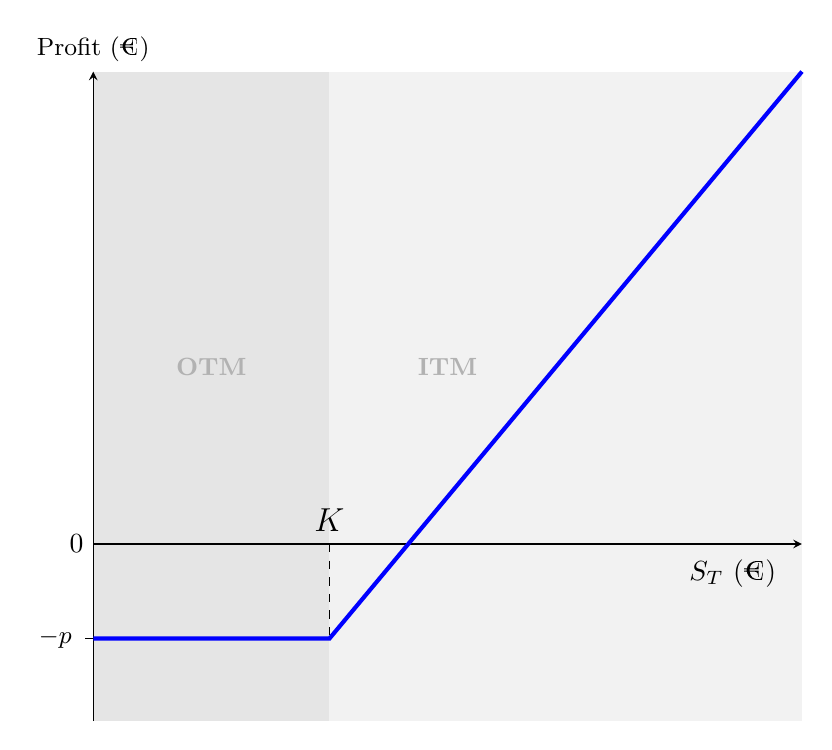
\begin{tikzpicture}[scale=1.5, >=stealth]

        % Shade area to the right of K (extending fully up to x-axis)
        \fill[gray!10] (2,-1.5) -- (6,-1.5) -- (6,4) -- (2,4) -- cycle;

         % Shade area to the left of K (extending fully up to x-axis)
        \fill[gray!20] (0,-1.5) -- (2,-1.5) -- (2,4) -- (0,4) -- cycle;


        % Define axes (extended x-axis)
        \draw[->] (0,0) -- (6,0) node[below,xshift=-25,yshift=-2pt, align=center] {$S_T$ (€)};
        \draw[->] (0,-1.5) -- (0,4) node[above] {\small Profit (€)};
        
        
        % Strike price line
        \draw[dashed] (2,0) -- (2,-0.8) node[above, yshift=35] {\large$K$};
        
        % Payoff function (thicker blue line)
        \draw[line width=1.5pt, blue] (0,-0.8) -- (2,-0.8) -- (6,4);
        
        % Marking zero level
        \node[left] at (0,0) {0};
        
        % Adding the premium annotation
        \draw (-0.07,-0.8) -- (0,-0.8); % Short tick line
        \node[left] at (-0.1,-0.8) {\small $-p$};

        % Add "ITM" label inside the fully shaded area
        \node[gray!60] at (3,1.5) {\small \textbf{ITM}};

        % Add "OTM" label inside the fully shaded area
        \node[gray!60] at (1,1.5) {\small \textbf{OTM}};

    \end{tikzpicture}
    \caption{Profit diagram for the long position in a call option. $K$ = strike price, $S_T$ = spot price, $p$ = premium. The buyer pays a premium to fix a maximum purchase price for the stock at a later point in time. At maturity, as long as $S_T < K$ there is no incentive to exercise the option, and the profit thus equals $-p$. The option is worthless, and is considered out of the money (OTM). When $S_T > K$, the option is in the money (ITM) and is assumed to be exercised as the buyer can now purchase the stock for $K$, immediately sell it for $S_T$, and offset some or all of the premium paid. However, the investment is only profitable once $S_T - K > p$.}
    \label{fig:long_call_payoff}
\end{figure}
\end{center}

The short call position exhibits an inverse profit profile compared to the long position: as long as the option remains OTM, the underwriter retains the full premium as profit, since the investor will not exercise the option. Once the option becomes ITM, the buyer will exercise it, forcing the underwriter to sell the stock at the strike price $K$ despite its higher market value $S_T$. The premium initially offsets this adverse price difference until the breakeven point where $S_T-K=p$, after which the position becomes a loss for the underwriter. Continuing with the previous example, this position could be taken by a crude oil producer with conviction that prices will remain below or near the strike price at maturity. The risk borne by the underwriter commands the premium. Figure~\ref{fig:short_call_payoff} illustrates this position.

\begin{center}
\begin{figure}[H]
\centering
    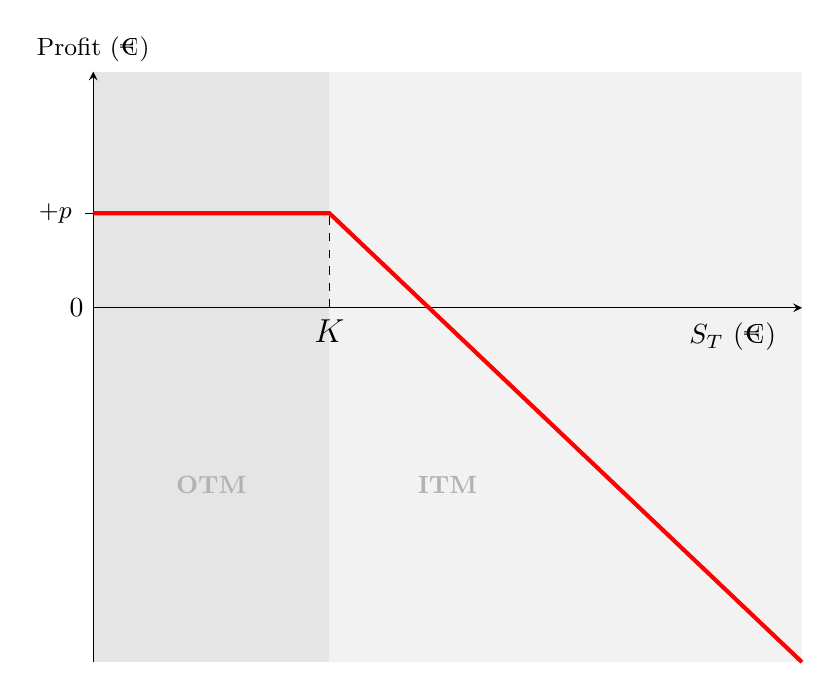
\begin{tikzpicture}[scale=1.5, >=stealth]
        % Create a more balanced diagram by shifting the origin up
        % Define y-range from -3 to +2 instead of -4 to +4
        
        % Shade area to the right of K
        \fill[gray!10] (2,-3) -- (6,-3) -- (6,2) -- (2,2) -- cycle;
        % Shade area to the left of K
        \fill[gray!20] (0,-3) -- (2,-3) -- (2,2) -- (0,2) -- cycle;
        
        % Define axes with shifted x-axis (moved up)
        \draw[->] (0,0) -- (6,0) node[below,xshift=-25,yshift=-2pt, align=center] {$S_T$ (€)};
        \draw[->] (0,-3) -- (0,2) node[above] {\small Profit (€)};
        
        % Strike price line
        \draw[dashed] (2,0) -- (2,0.8) node[below, yshift=-35] {\large$K$};
        
        % Payoff function (thicker red line for short position)
        \draw[line width=1.5pt, red] (0,0.8) -- (2,0.8) -- (6,-3);
        
        % Marking zero level
        \node[left] at (0,0) {0};
        
        % Adding the premium annotation
        \draw (-0.07,0.8) -- (0,0.8); % Short tick line
        \node[left] at (-0.1,0.8) {\small $+p$};
        
        % Add labels inside the shaded areas
        \node[gray!60] at (1,-1.5) {\small \textbf{OTM}};
        \node[gray!60] at (3,-1.5) {\small \textbf{ITM}};
    \end{tikzpicture}
    \caption{Profit diagram for the short position in a call option. $K$ = strike price, $S_T$ = spot price, $p$ = premium. The underwriter receives a premium but is obligated to sell the stock for $K$ at a later time point, should the option be exercised. When $S_T < K$, the option is worthless and considered out of the money (OTM), allowing the underwriter to keep the full premium as profit. When $S_T > K$ and the option is exercised in the money (ITM), the underwriter is forced to sell the stock at the strike price $K$ despite its higher market value $S_T$. The profit decreases linearly as $S_T$ increases, becoming negative once $S_T - K > p$.}
    \label{fig:short_call_payoff}
\end{figure}
\end{center}


Ignoring the premium, the payoff from the long position in a call option is defined as
\begin{equation}
    \max(S_T-K,0)
\end{equation}
as the investor will only exercise when ITM to either profit or offset losses. The payoff from the short position is defined as
\begin{equation}
    -\max(S_T-K,0) = \min(K-S_T,0)
\end{equation}
due to the zero-sum nature of the contract \cite[p. 9]{hull2016options}.\footnote{For American-style options with the right to early-exercise, the payoff is calculated using $S_\tau$ instead of $S$, where $\tau \le T$ is the chosen exercise time.}

\subsubsection{Put Option Positions}
The investor is willing to pay a premium up front in order to fix a price for selling a later time. In other words, they expect the price of the underlying asset to decrease enough to offset this premium. Meanwhile, the underwriter receives a premium but is obligated to engage in this potential future trade, and thus expects the price not to decrease too much from the market price. Figure ~\ref{fig:put_payoff} depicts the profit diagrams of the long and short positions of a put option:


\begin{figure}[H]
    \makebox[\textwidth][c]{
    \hspace{-1cm} % Fine-tune centering
    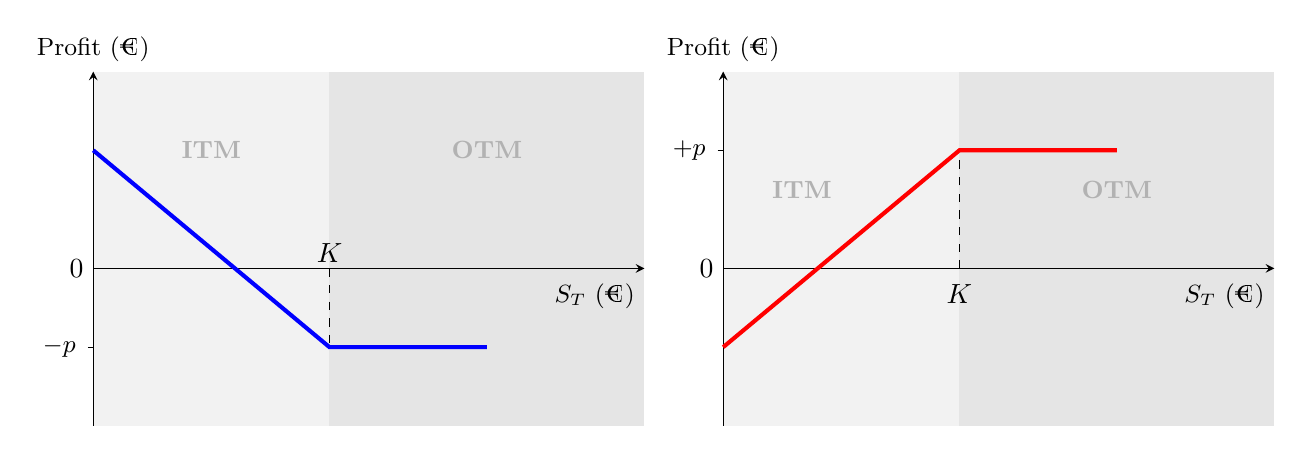
\begin{tikzpicture}[scale=1, >=stealth]

     % Left Diagram: Long Put
    \begin{scope}[shift={(-0.5,2)}]  % Shifted slightly left

        % Shade area to the right of K (OTM for long put)
        \fill[gray!20] (3,2.5) -- (7,2.5) -- (7,-2) -- (3,-2) -- cycle;

        % Shade area to the left of K (ITM for long put)
        \fill[gray!10] (0,2.5) -- (3,2.5) -- (3,-2) -- (0,-2) -- cycle;

        % Define axes
        \draw[->] (0,0) -- (7,0) node[below,xshift=-18,yshift=-2pt, align=center] {\small$S_T$ (€)};
        \draw[->] (0,-2) -- (0,2.5) node[above] {\small Profit (€)};
    
        % Strike price line
        \draw[dashed] (3,0) -- (3,-1) node[above, yshift=27] {$K$};
    
        % Payoff function (thicker blue line for long put)
        \draw[line width=1.5pt, blue] (0,1.5) -- (3,-1) -- (5,-1);%(0,1.5) -- (2,1.5) -- (5,-1);

        % Marking zero level
        \node[left] at (0,0) {0};
    
        % Adding the premium annotation
        \draw (-0.07,-1) -- (0,-1); % Short tick line
        \node[left] at (-0.1,-1) {\small $-p$};

        % Add "ITM" label inside the shaded area (long put ITM is left of K)
        \node[gray!60] at (1.5,1.5) {\small \textbf{ITM}};

        % Add "OTM" label inside the shaded area (long put OTM is right of K)
        \node[gray!60] at (5,1.5) {\small \textbf{OTM}};

    \end{scope}

    % Right Diagram: Short Put (Shifted slightly left from 9 to 8)
    \begin{scope}[shift={(7.5,2)}]  

        % Shade area to the right of K (ITM for short put)
        \fill[gray!20] (2,2.5) -- (7,2.5) -- (7,-2) -- (2,-2) -- cycle;

        % Shade area to the left of K (OTM for short put)
        \fill[gray!10] (0,2.5) -- (3,2.5) -- (3,-2) -- (0,-2) -- cycle;

        % Define axes
        \draw[->] (0,0) -- (7,0) node[below,xshift=-18,yshift=-2pt, align=center] {\small$S_T$ (€)};
        \draw[->] (0,-2) -- (0,2.5) node[above] {\small Profit (€)};
    
        % Strike price line
        \draw[dashed] (3,0) -- (3,1.5) node[below,yshift=-45] {$K$};
    
        % Payoff function (thicker red line for short put)
        \draw[line width=1.5pt, red] (0,-1) -- (3,1.5) -- (5,1.5);

        % Marking zero level
        \node[left] at (0,0) {0};
    
        % Adding the premium annotation
        \draw (-0.07,1.5) -- (0,1.5); % Short tick line
        \node[left] at (-0.1,1.5) {\small $+p$};

        % Add "OTM" label inside the shaded area (short put OTM is right of K)
        \node[gray!60] at (5,1) {\small \textbf{OTM}};

        % Add "ITM" label inside the shaded area (short put ITM is left of K)
        \node[gray!60] at (1,1) {\small \textbf{ITM}};

    \end{scope}

    \end{tikzpicture}

    
}
\caption{Profit diagrams: (Left) Long put option, (Right) Short put option.}
\label{fig:put_payoff}
\end{figure}

A put option is worthless (OTM) when $S_T > K$ as the investor will not exercise it to sell for a lower price than market value. By the same token, the option is ITM when  $S_T < K$, as the investor can then buy the underlying asset at market value and sell it for the strike price \cite[p. 209]{hull2013fundamentals}. Again, being ITM is not sufficient to be profitable - the price difference must be large enough to offset the paid premium.

An example use case would be a crude oil supplier forecasting low prices in a year's time and entering the long position to secure a minimum revenue. Again, a premium is paid to hedge against a risk of price swings. The short side would be taken by a market participant who expects crude oil prices not to fall enough to offset the received premium.
\bigskip

The payoff from the long position in a put option is defined as

\begin{equation*}
    \max(K-S_T,0)
\end{equation*}

as being ITM now means $K > S_T$. The payoff in the corresponding short position is

\begin{equation}
    -\max(K-S_T,0) = \min(S_T-K,0)
\end{equation}

due to the zero-sum nature of the contract \cite[p. 10]{hull2016options}.

The long position in any option contract is never obligated to exercise, and the loss is therefore limited to the premium paid. On the other hand, the underwriter is always obligated to engage in a disadvantageous trade with the buyer. This, combined with the fact that underlying asset prices have no theoretical upper bound, whereas they are (in most cases) limited to non-negative values, makes taking the short position inherently more risky. Figure \ref{fig:optiontable} aggregates information about the extreme-case profit and loss incurred from the different option types and positions.



\begin{figure}[htbp]
\centering
\label{options-risk-table}
\begin{tabular}{|l|p{5cm}|p{5cm}|}
\hline
\textbf{Position} & \textbf{Call Options} & \textbf{Put Options} \\
\hline
\textbf{Long} & \textbf{Maximum Gain:} $+\infty$
\newline \textbf{Maximum Loss:} $-p$ & \textbf{Maximum Gain:} $K-p$
\newline \textbf{Maximum Loss:} $-p$ \\
\hline
\textbf{Short} & \textbf{Maximum Gain:} $+p$
\newline \textbf{Maximum Loss:} $-\infty$ & \textbf{Maximum Gain:} $+p$
\newline \textbf{Maximum Loss:} $-(K-p)$ \\
\hline
\end{tabular}
\caption{Risk profiles for different option positions. $p$ = premium paid/received, $K$ = strike price. Long calls have unlimited upside potential due to theoretically unbounded asset prices, with losses limited to the premium paid. Short calls mirror this with unlimited downside risk. Put options have bounded payoffs as asset prices cannot fall below zero, with maximum gain for long puts at $K-p$ (when spot price reaches zero) and maximum loss for short puts at $-(K-p)$.}\label{fig:optiontable}
\end{figure}

The objective of pricing models is to find the so-called fair value of the option~$p$. Although market prices form through the dynamic interaction of buyers and sellers, they are still to a large extent based on theoretical pricing frameworks. These models provide a rational foundation for valuing derivatives based on mathematical and economic theory. While real-world prices may show short-term deviations, markets tend to converge toward theoretically justified values over time, as persistent mispricing creates exploitable opportunities. The theoretical fair value serves as a crucial reference point that informs trading decisions and risk management strategies.


\subsection{Price Determinants and Sensitivity}

Hull et al. \cite{hull2013fundamentals} define six factors influencing the price of the option. While these often make up the variables in our pricing models, one can intuitively reason about their effect in a model-free context. This also, however, provides some explanation on why they appear in the models in the first place. They are presented in a ``ceteris paribus'' context, or all else being equal. This is rarely the case in practice, however, as markets quickly incorporate available information into prices \cite{fama1970efficient}. The underlying asset price is consequently affected by changes in some of the factors. For clarity, we are considering the long position, i.e. the perspective of the buyer.

The stock price relative to the strike price is perhaps the most obvious factor. The effect on the payoff is thoroughly explained in subsection ~\ref{payoffs}, and the price naturally increases with the payoff. Thus, the price of a call option increases with the underlying asset, while the inverse relationship is observed for a put option.

Volatility, a statistical measure of the variation in asset prices over a specific time period, has a positive effect on both call and put options. This can be motivated by the limited downside -- unlimited upside nature of options (see figure \ref{fig:optiontable}), which makes larger price movements more advantageous as it increases the probability of moving ITM. This is especially obvious for OTM positions, where a price movement is still needed in order not to expire worthless, but holds for ITM positions as well, as the unlimited potential for becoming even deeper ITM outweighs the limited downside of going OTM.

Time to maturity has a more complex relationship with the price, and depends on both the option style and the context. For American-style options where early exercise is allowed, it makes sense that an expiration date further in the future leads to more opportunity for favorable movements in the underlying, thereby commanding a higher price. This is effectively the same argument as was made for volatility. While this so called "time-decay" argument also holds for European-style options, the lack of early-exercise complicates the matter. There exist specific scenarios where one would benefit from exercising the option earlier. The authors propose the example of a future dividend payment to the shareholders of the underlying company, which theoretically decreases the share price and thereby the value of the corresponding call option. An example of a put option being of higher value with a shorter timer to maturity would be the case of a very deep ITM position, e.g. if the company of the underlying asset has filed for bankruptcy. The option will almost certainly expire ITM, and thus by the \textbf{time value of money} principle this cash flow is worth more the earlier it is received \cite[pp. 97-101]{berk2007corporate}.


The risk-free rate represents the return on investment one can expect from a so called risk-free investment. In practice, this means some form of government-backed treasury bill (as the government is "too big to fail"). It often serves as a sort of benchmark measurement to which investors compare the expected rates of return of other, riskier investments. Given a risk level for an investment, an increase in the risk-free rate leads to investors expecting a higher return on said investment. Consequently, since the expected rate of return is often used as the discount rate for obtaining the present value of future cash flows, it decreases the present value of the strike price, which, all else being equal, is a better deal for the buyer and increases the value of the call option. By the same token, the value of a put option decreases, as the strike price is "worth more" by maturity than what it is in today's money. In practice, however, interest rates tend to have a notable and varying impact on different underlying asset prices as well, so this is more of a theoretical relationship assuming a standard share as the underlying.

The final determinant considers the dividend policy of the underlying asset (stock). Theoretically, a company's share price is reduced by the dividend, as this money is directly deducted from the cash flows that make up the value of the equity in the first place \cite{modigliani1958cost}. Thus, a dividend payment policy decreases the value of a call option, and increases the value of a put option.

In addition to pricing the option, traders and risk managers alike are often interested in measuring how sensitive this price is to changes in these determinants. Model imperfections make it desirable to understand the effect of small perturbation in the variables, hence these often play a significant role in different hedging and trading strategies \cite{hull2016options}. These sensitivity calculations often require additional computational effort beyond basic option pricing, as each Greek may require re-evaluating the pricing model with perturbed inputs or calculating complex partial derivatives. In practice, risk management systems need to calculate both prices and multiple Greeks for thousands of options simultaneously, substantially increasing computational demands and making GPU acceleration particularly valuable \textbf{(do I need src for this?????)}. \textbf{(maybe I need to state something here about the later chapters also having a look at how these can be computed efficiently alongside the price. But depends on what the sources have to say)}. Wilmott \cite{wilmott2013paul} defines the following five main sensitivity measures, also known as \emph{the Greeks}, with respect to the aforementioned determinants. Let $V$ be the price (value) of the option, $S$ the underlying asset price, $t$ the time to maturity, $r$ the risk-free rate, and $\sigma$ the volatility of the underlying asset. A high-level definition of the Greeks is:
\begin{align*}
    \Delta &= \frac{\partial V}{\partial S} & \text{(Delta: sensitivity to changes in the underlying price)} \\[0.5em]
    \Gamma &= \frac{\partial^2 V}{\partial S^2} & \text{(Gamma: rate of change of Delta, or convexity)} \\[0.5em]
    \Theta &= \frac{\partial V}{\partial t} & \text{(Theta: sensitivity to the passage of time)} \\[0.5em]
    \nu &= \frac{\partial V}{\partial \sigma} & \text{(Vega: sensitivity to volatility changes)} \\[0.5em]
    \rho &= \frac{\partial V}{\partial r} & \text{(Rho: sensitivity to changes in the risk-free rate)}
\end{align*}

Note that the formal definitions of the Greeks are model-specific. The choice to represent them using partial derivatives suggests the context of a continuous-time model, and these are indeed defined in relation to the BSM model. Nevertheless, this formulation provides an intuitive understanding of the measurements. In discrete-time models (like CRR) or discretized approximations of BSM, the Greeks are redefined or estimated using different techniques (do I need sources???).


\subsection{No-Arbitrage Pricing and the Replicating Portfolio ??? Risk-Neutrality}
Previously, all main "ingredients" for our pricing formulas were introduced. This section outlines the foundational theoretical framework that underpins all option pricing models, and moves one step closer to formulating the models which we want to implement. In line with the scope, the focus will be on intuition as opposed to rigor. Avid readers are encouraged to explore the references in greater detail (WHICH ONES SPECIFICALLY???). We continue with the common set of assumptions that maintains the theory, such as no transaction costs and perfectly liquid markets.

A starting point would be to draw inspiration from the arguments used when pricing other assets. We often consider the theoretical value of an asset as the discounted sum of all future cash flows it produces. In case of uncertainty (as is the case of all risky assets) it is not an unreasonable idea to discount the \emph{expected value} these cash flows instead, as it represents a theoretical long-term average of the returns \textbf{(basic math and financial theory, do I need src for this?)}. Calculating this expected value, however, requires defining a set of possible outcomes (returns) and assigning a probability to each one of them. This is often the limitation of pricing models in general, as the guesstimates are questionable and varies with people's risk preferences. Nonetheless, starting out with a simplistic model will lead to interesting and useful revelations that can be expanded on. This setup considers European-style options.

The \emph{no-arbitrage principle} is the essential assumption for what is to come. Arbitrage describes the act of simultaneous buying and selling the same asset in different markets to make risk-free profit off price differences. Imagine the price of tomatoes being higher in one of two neighboring towns. Perhaps the tomato farmers were really successful in town A this year, and the increased supply dropped the prices somewhat. This information has not yet been priced into the tomatoes in town B. The adroit tradesman could then buy tomatoes in town A and immediately sell them in town B to pocket the difference, without taking any position on future tomato price movements. This, again, assumes ideal conditions, like enough liquidity to always be able to both buy and sell, as well as ignoring friction costs like transportation. The idea behind our assumption is that this situation ultimately is self-eliminating: as the tradesman continues to introduce more tomatoes to the total supply in town B they will drive the price down until an equilibrium has been reached. Other people may take notice, and decide to adopt the same strategy, eliminating the opportunity even faster. The information of the increased supply in town A has now been priced into the tomatoes in town B. This example is not too far-fetched from reality. Modern digital markets, while not perfectly adhering to the assumptions laid out above, form an environment where short-term arbitrage opportunities can exist. Nevertheless, as sophisticated market participants exploit these market inefficiencies they quickly disappear due to subsequent price corrections. Thus, the no-arbitrage principle is a reasonable assumption, at least over longer time periods. If our pricing methodology is based on future cash flows it logically follows that in absence of arbitrage opportunities two assets producing the same cash flows must be priced equally (DO I NEED SRC FOR THIS?????).

If then, it were possible to find an existing asset with identical cash flows as the option itself, whose price is already known, that should theoretically equal the price of the option. Hull et al. \cite{hull2013fundamentals} consider a one-step binomial model as the simplest setup to utilize this assumption. In this discrete-time model we consider the underlying asset price's evolution over one time-step. This will be presented in a slightly different manner. Let $S_0$ be the current price of an asset, and $f$ the current price of an option on this underlying asset, with time $T$ to maturity. The underlying price is restricted to two future states: $S_0u$ or $S_0d$ ($u>1$, $d<1$), each corresponding to the option payoffs $f_u$ and $f_d$. Figure \ref{fig:oneperiodbinom} visualizes the model setup. This restriction allows for creating a so-called \emph{replicating portfolio} that fully matches the payoff structure of the option. This portfolio consists of $\Delta$ shares of the underlying asset, as well as $B$ amount of a risk-free asset, for example money in a savings account, appreciating in value by the risk-free rate $r$. After time period $T$ our portfolio can be in two states, depending on if the underlying asset price increased or decreased. Equating these with the corresponding option payoffs obtains two equations with two unknown variables, $\Delta$ and $B$:

\begin{equation}
\begin{cases}
    \Delta (S_0u) + B(1+r) = f_u\\
    \Delta (S_0d) + B(1+r) = f_d
\end{cases}
\end{equation}
Solving for these variables yields

\begin{equation}
    \Delta = \frac{f_u - f_d}{S_0(u-d)}
\end{equation}
\begin{equation}
    B = \frac{f_du-f_ud}{(u-d)(1+r)}
\end{equation}

It is evidently possible to construct a portfolio with identical payoff structure as the option itself, according to


\begin{equation}
     \frac{f_u - f_d}{S_0(u-d)} S_0 + \frac{f_du-f_ud}{(u-d)(1+r)}
\label{eq:replicating-portfolio}
\end{equation}


Assuming no-arbitrage (along with other assumptions like perfect capital markets, no transaction costs, no taxes, no dividends ? ..., ), the price of the option must thus equal the price of constructing the replicating portfolio (i.e. buying $\Delta$ shares and investing $B$ in a risk-free asset). Otherwise, one could buy the cheaper alternative while selling the more expensive to obtain a risk-free profit. A negative $\Delta$ implies shorting the underlying asset (do I need footnote for shorting?), and a negative $B$ implies borrowing money at the risk-free rate instead of lending (saving) it.

\begin{figure}[h]
    \centering
    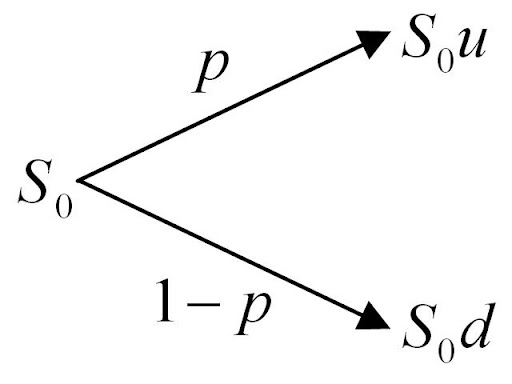
\includegraphics[width=0.5\textwidth]{oneperiodbinom.jpg}
    \caption{Graphical representation of the one-period binomial option pricing model. REPLACE WITH YOUR OWN VERSION, MAKE TEXT BETTER, ALSO INCLUDE THE CALL OPTION UP AND DOWNS}
    \label{fig:oneperiodbinom}
\end{figure}



There are several interesting points to note about this result: firstly, note that $\Delta$, representing the amount of shares to hold or short, can also be mathematically thought of as the ratio of the range of option prices at maturity to the range of the underlying prices at maturity. The choice of notation is deliberate, as this is precisely the one-step discrete version of the delta Greek introduced earlier. Secondly, note that the derivation assumed neither call nor put, and functions therefore as a pricing model for any European-style option. Perhaps the most interesting observation, however, is the fact that this pricing approach contains no information about the expected return of the underlying, or the probability with which it will rise/fall in value. The authors motivate this intuitively by the fact that such expectations are already reflected in the price of the underlying, and need not be explicitly accounted for. The option is priced relative to the underlying asset.

This also leads to the fundamental concept of \emph{risk-neutral} valuation. Rearrange \ref{eq:replicating-portfolio} into

\begin{equation}
     \frac{1}{1+r}\left(f_u(\frac{(1+r)-d}{u-d})+f_d(\frac{u-(1+r)}{u-d})\right)
\end{equation}

. Let $\tilde p := \frac{(1+r)-d}{u-d}$ be the probability of an up move, and  $\tilde q := \frac{u-(1+r)}{u-d}$ the probability of a down move. The no-arbitrage assumption imposes $d \leq (1+r) \leq u$, which leads to $0 \leq \tilde p \leq 1$ and  $0 \leq \tilde q \leq 1$ (https://quant.stackexchange.com/questions/55239/explaining-the-risk-neutral-measure) OR (https://web.ma.utexas.edu/users/mcudina/m339d-lecture-17-binomial-option-pricing-one-period.pdf). Furthermore, $\tilde p + \tilde q = 1$ (quant stack citation???). These can be interpreted as risk-neutral probabilities, and thus the option can be priced as the expected payoff under this new probability measure, discounted at the risk-free rate. One can think of risk-neutral valuation as a convenient mathematical reformulation. By considering the equivalent situation in an alternative reality where market participants are assumed to be risk-neutral (which clearly does not hold in our reality \cite{kahneman2013prospect}) one obtains a more familiar framework for valuing assets by considering their discounted expected cash flows. This elegant reformulation enables the use of powerful tools from probability theory. For these reasons, the risk-neutral approach is widely adopted in modern option pricing, and elements of it will be found in all of the models to be introduced later. \cite{gisiger2010risk} \cite{tham2001risk}

\begin{equation}
     \frac{1}{1+r}(f_u\cdot \tilde p + f_d \cdot (1-\tilde p))
\label{risk-neutral-expectancy}
\end{equation}




\section{The GPU and Parallel Computing} \label{sec:gpu}
The graphics processing unit (GPU) is a processor specified for graphics-related processing. Starting in the 1980s, the demand for 2D and 3D graphically based consumer software, mainly driven by video games, surged. In practice, this entailed performing a large amount of floating-point operations per seconds (FLOPS) associated with graphical operations like shading and rasterization. Front-runners of delivering affordable graphics computing capabilities included NVIDIA and ATI Technologies (later acquired by Advanced Micro Devices (AMD)).\cite{sanders2010cuda} \cite{kirk2016programming}

Hennessy and Patterson \cite{hennessy2011computer} loosely define \emph{latency} as the time between the start and completion of a single event, and \emph{throughput} as the total amount of work performed in a given time. These metrics (and specific variants thereof) are widely used in computing performance contexts. While both central processing units (CPUs) and GPUs have seen performance improvements on both ends, the authors show that relative throughput improvements tend to outweigh relative latency improvements. This is not unreasonable - increasing throughput is (within limits) mostly a manner of providing more of the same resources already available. Latency improvements have, on the other hand, already reached closer to the theoretical limits imposed by the laws of physics \cite{hennessy2011computer} \cite{sanders2010cuda}. Suomela's summary of statistics on trends for both clock speed and instruction latencies corroborate these claims (cite PPC website?).

This, in combination with the fact that graphics-related calculations are well-structured for concurrency exploitation (covered in section \ref{subsec:parallell}), led to the evolution towards the exceptionally throughput-optimized GPU architectures of today's age. At the same time, there grew an increasing interest in the utilization of these parallel computing capabilities for other purposes. However, these advances alone were insufficient in unlocking the potential for so called general-purpose GPU (GPGPU) programming, as the hardware lacked the flexibility needed for general-purpose computing, and no GPGPU programming models and tools were readily available. The initial graphics-intended hardware and software ecosystems effectively forced developers to mask their problems as those found in the graphics domain. Only after advances in these areas could GPGPU programming truly flourish. In 2007, NVIDIA released the compute unified device architecture \emph{CUDA} and corresponding software tools that greatly removed earlier restrictions in favor of GPGPU-programming. The hardware was now directly accessible without considering graphics-related interfaces, and the software tool for writing CUDA applications was a simple extension layer on top of familiar C/C++. Today, GPGPU applications are found in a wide variety of fields, including computational finance. \cite{sanders2010cuda} \cite{kirk2016programming}

\subsection{CPU and GPU Architecture}

Figure \ref{fig:CPUandGPU} represents a very simple model of a modern CPU and GPU. The \emph{arithmetic logic unit} (ALU) is responsible for performing bitwise operations on data, \emph{registers} (not explicitly visible in figure) for storing memory addresses, instructions, and data to operate on, as well as additional supporting components, e.g. for control of flow, or communication with the external environment. The CPU operates in a loop of two-staged fetch-execute instruction cycles, where an instruction is first loaded into the so-called instruction register. After this, the instruction is decoded and executed, which in practice means either data processing, data transfer, or control logic related to the instruction sequence. This loop continues until the program halts due to either finishing or due to an interruption by another module.\cite{stallings2011operating}

CPUs have with time adapted to improve performance by utilizing various parallelism mechanisms. Instruction-level parallelism (ILP) refers to a set of techniques the processor uses for executing multiple instructions, either in part or fully, simultaneously. Common examples of these are pipelining, branch prediction and speculative execution. Processor architectures often contain \emph{single instruction multiple data} (SIMD) capabilities through large vector registers capable of storing multiples of the same data type, and instructions that can operate on these at once. And to top it off, most modern processors are multi-core, meaning they literally contain multiple instances of the main aforementioned components for use. This enables a higher thread-level parallelism (TLP), where a \emph{thread} — informally defined as an independent sequence of instructions that can be scheduled and executed as a separate unit of work \textbf{do I need src??} — can run on each core simultaneously. Despite this, the CPU remains primarily latency-optimized, and does not hold a candle to the typical GPU throughput. \cite{hennessy2011computer}

\begin{figure}[h]
    \centering
    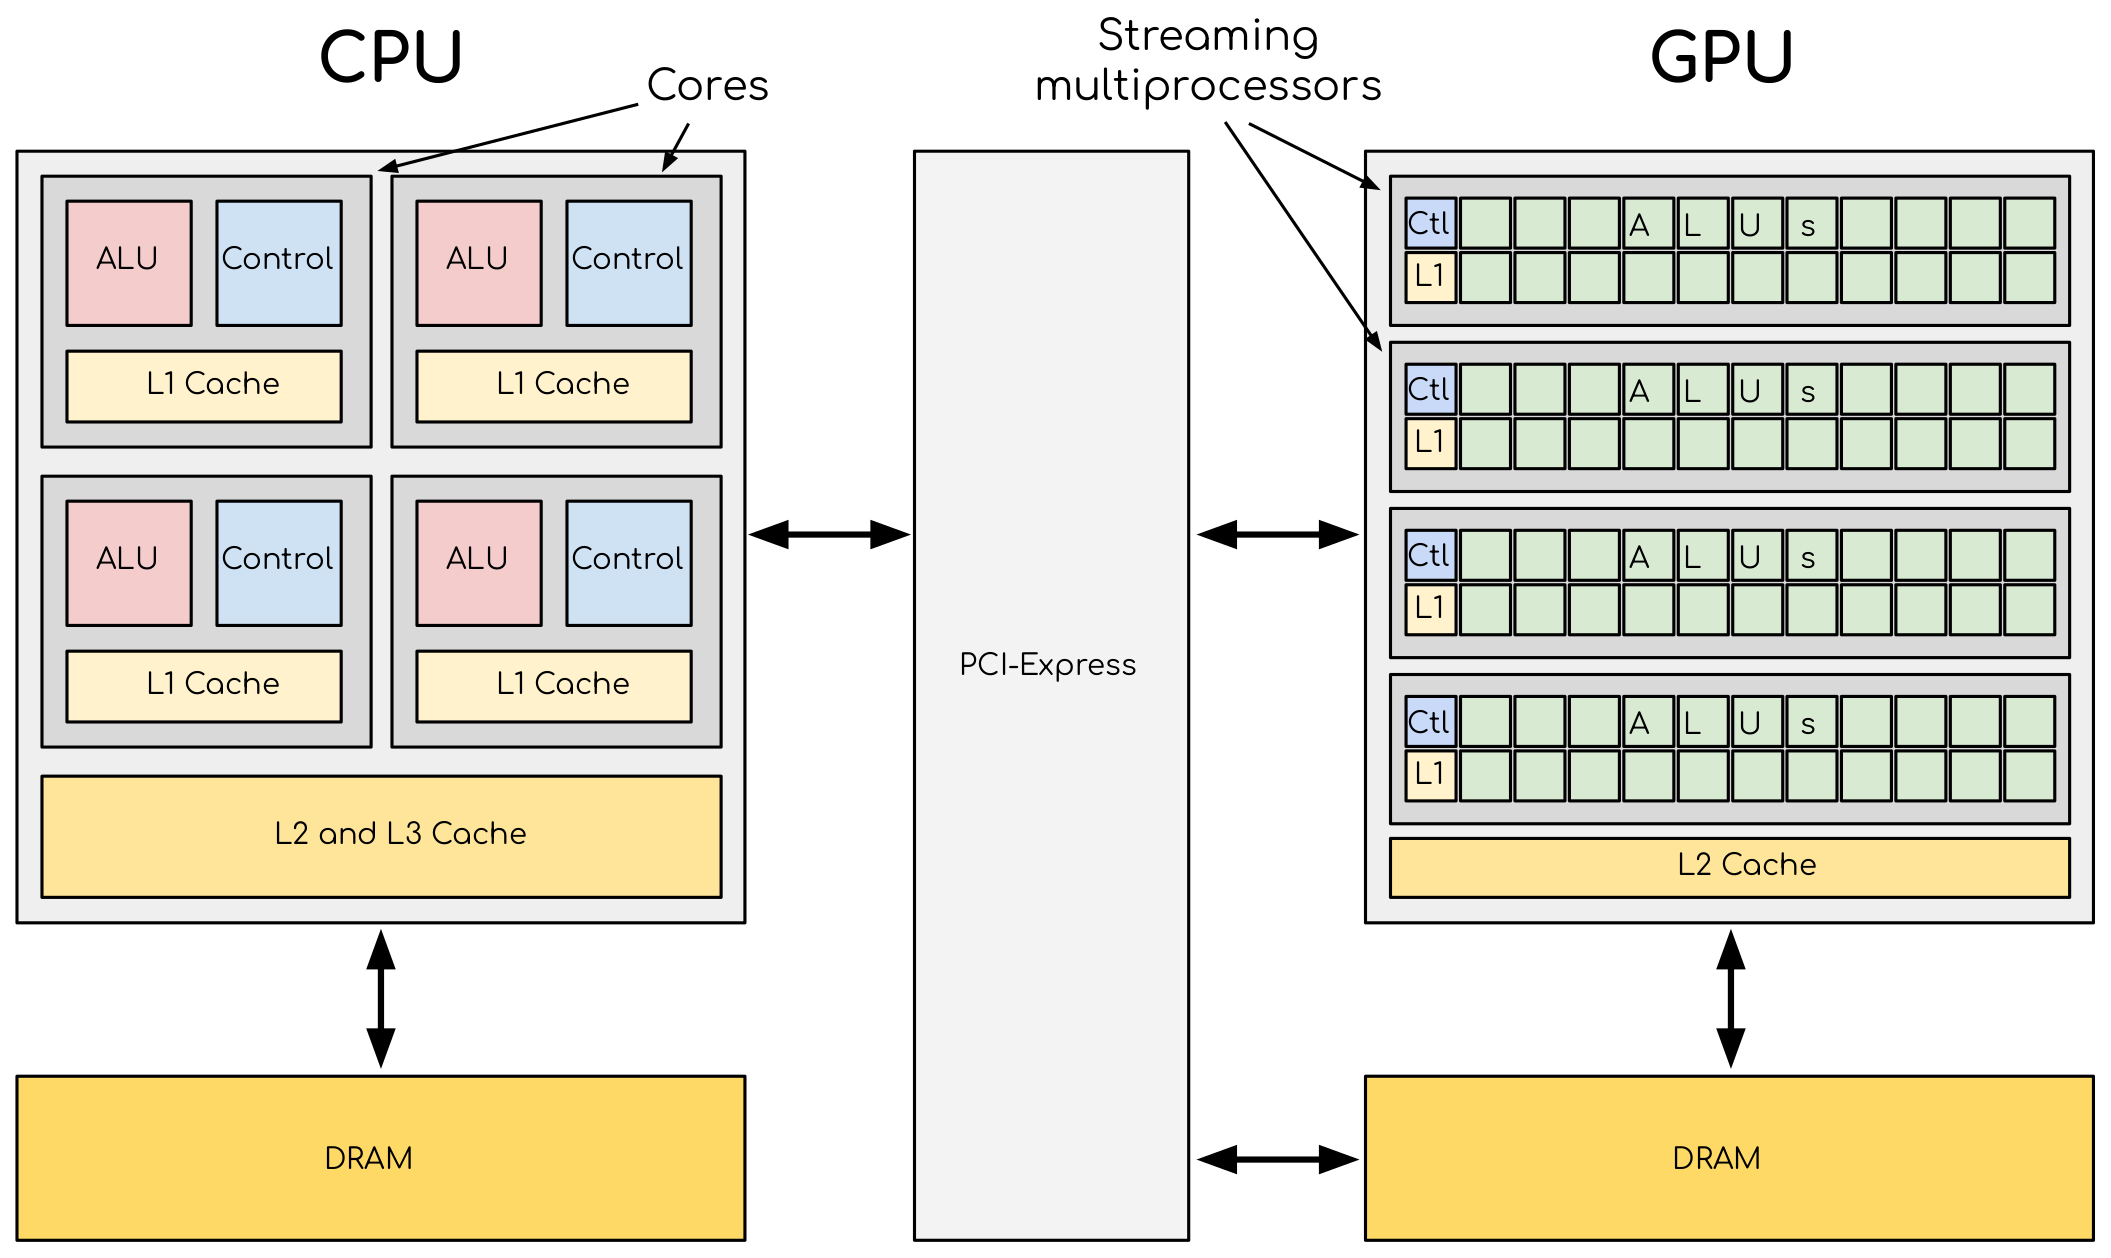
\includegraphics[width=0.8\textwidth]{CPUAndGPU.png}
    \caption{Simple diagrams of modern multi-core CPU and GPU architectures, showcasing their main respective components. Each CPU core contains an arithmetic logic unit (ALU) for performing bitwise operations and a control unit for handling program flow. Hierarchical (L1-L3) on-chip cache memory minimizes data transfer bottlenecks between the (D)RAM and the cores. On the GPU, streaming multiprocessors correspond to cores. The design clearly emphasizes parallel computing power over control and latency optimization. The PCI-Express serves as a data transfer interface between the processors. source: https://enccs.github.io/gpu-programming/2-gpu-ecosystem/ OK TO DO THIS??}
    \label{fig:CPUandGPU}
\end{figure}

In contrast, while lacking many of the sophistication that makes the CPU excel at sequential and "control-complex" tasks, the GPU fits in more raw computation power for a massively throughput-optimized architecture that excels at the specialized task of parallel numerical computation. The term single instruction multiple thread (SIMT) is often used to describe GPU computation, as the concurrency is enabled on thread-level by a massive amount of threads running scalar computations in parallel, as opposed to single-threaded computation using SIMD and ILP methods (or multi-threaded on a comparatively few cores). Suomela (cite PPC) has nicely summarized these differing parallelism paradigms. A modern CUDA-based GPU containing many independent \emph{streaming multiprocessors} (SM), which can be considered as a group of many \emph{streaming processors} (SP) (read: ALUs) sharing some control units and instruction memory registers. Threads are grouped in to groups of 32, called \emph{warps}, which always execute in lock-step, i.e. simultaneous execution on their respective data. The threads in a warp are thus dispatched to a corresponding amount of SPs using these shared resources. Similarly to a multi-core CPU, all SMs share a higher-latency global memory (akin to RAM), and are individually allocated a small but fast on-chip cache for minimizing data transfer bottlenecks, among other things (to be discussed later). \cite{sanders2010cuda} \cite{kirk2016programming} (cite PPC)



\subsection{Parallel Computing Fundamentals and GPU suitability}\label{subsec:parallell}

Types of parallelism (data, task, instruction)
Amdahl's Law and theoretical speedup limits
Dependency chains and their impact
Synchronization requirements
Characteristics of "GPU-friendly" algorithms
Identifying parallelizable components
MAKE POINT THAT GRAPHICS CALCULATIONS ON PIXESL ETC WERE LARGELY PARALLELIZABLE DUE TO LOW DEPENDENCY CHAINS  
Common computation patterns in finance
Performance metrics and evaluation






\subsection{(GP)GPU Programming Model}



add * footnote explaining warps vs blocks, link to Suomela PPC
Thread hierarchy (threads, blocks, grids)
Memory spaces (global, shared, constant, texture)

-> WHY THIS? difference between logical view vs hardware view. Logical for structuring problem (indexing) according to its "natural dimensions" better, and hardware independence no matter how many SMs available et.c. + shared memory constructs for synching work!




Hardware-Level Concerns (Managed by GPU)

Warp formation and execution (32 threads in lockstep)
Warp scheduling on available SMs
Thread masking during branch divergence
Memory coalescing at warp level
Register allocation per thread
L1/L2 cache management
SM resource allocation
Load balancing across SMs

Programmer-Level Concerns (Your Focus)

Block and grid dimensions that match problem structure
Thread indexing within problem domain
Shared memory allocation and usage
Managing data transfers between CPU and GPU
Minimizing thread divergence
Optimizing memory access patterns
Balancing resources per thread/block
Maximizing occupancy (concurrent warps)
Synchronization between threads when needed
Decomposing problem into parallel components

The key insight is that programmers think in terms of the problem structure (blocks/grids), while the hardware manages the execution details (warps/SMs). This separation of concerns is what makes CUDA both powerful and accessible.RetryClaude can make mistakes. Please double-check responses.





Execution model and scheduling
CUDA programming paradigm

\subsection{WHY GPU?} the need for computational power:

This is a crucial question that gets to the heart of why GPU acceleration is valuable in option pricing. The justification comes from several real-world financial applications:

Risk Management: Financial institutions need to calculate Value-at-Risk (VaR) and other risk metrics for portfolios containing thousands of options. This often requires:

Recalculating all option prices under multiple scenarios
Computing Greeks to understand sensitivity to market movements
Running these calculations daily or even intraday


Regulatory Requirements: Banking regulations like Basel III require comprehensive stress testing of portfolios, involving:

Calculating option values under hundreds of different market scenarios
Reporting results within strict timeframes


Electronic Market Making: Firms that provide liquidity in options markets need to:

Continuously update prices for hundreds or thousands of options
Adjust their quotes as market conditions change
Maintain accurate hedging calculations (based on Greeks)


Portfolio Optimization: Investment firms need to:

Evaluate complex trading strategies across multiple options
Test different portfolio compositions
Optimize hedging positions using sensitivity metrics



This computational demand is documented in various sources:

Academic papers like "GPU Computing in Finance: Recent Applications and Developments" by Giles \& Xiaosong (2014) discuss these requirements
Financial industry whitepapers from firms like NVIDIA and JP Morgan
Case studies from banks that have implemented GPU solutions for options pricing

The computational demands become especially intense during market stress when quick recalculation is critical, making the case for GPU acceleration even stronger.



- why GPU, why optimize for throughput vs latency


\clearpage

\section{GPU Acceleration of the Cox-Ross-Rubinstein Binomial Model} \label{sec:gpu-crr}

The CRR model extends the idea of the one-period binomial model into its multi-period counterpart. Again, by assuming discrete time-periods and constant factors u and d, one obtains a larger set of final states for the price of the underlying, as well as for the option payoff. One can now recursively backtrack the tree by starting at the final state nodes and, using the one-period model, calculating the value of the option (i.e. the value of the replicating portfolio) at each node until we obtain the initial price at t=0. For simplicity, the risk-neutral expected payoff formula (\ref{risk-neutral-expectancy}) is used, and the tree thus models the underlying asset price in the risk-neutral world. \cref{fig:combined} visualizes this idea. \cite{cox1979option}

A so far omitted detail has been the choice of the factors $u$ and $d$. The authors of the original paper have defined $u = e^{\sigma\sqrt{t/n}}$ and $d = e^{-\sigma\sqrt{t/n}}$, where $\sigma$ is the annualized volatility (e.g. estimated from historical data) of the (log-return of) the asset, $t$ is the time of the entire period (in years), and $n$ is the number of sub-intervals. This is useful for several reasons: firstly, it allows for the model to converge to the famous BSM model as $n \rightarrow \infty$. Secondly, the tree recombines for all permutations of a price path, allowing for feasible computational requirements. Another detail to note is that the discount rate used in the sub-interval calculations must be adjusted such that it yields the same return as the initial risk-free rate used in the one-period example. A continuous compounding rate $e^{rt/n}$ is often used in lieu of the discrete version. \cite{cox1979option} \cite{hull2013fundamentals}

The implementation of the CRR model for European-style options comprises three steps: first, compute the price of the underlying at all the terminal nodes. Then, calculate the corresponding option payoffs for the terminal nodes. Finally, backtrack the option payoff tree and recursively compute its value at the end of the previous period using the current "final states". The following pseudocode is based on the Python implementation by TheQuantPy [how to cite GitHub?]. Let $S_0$ be the initial underlying (stock) price and $n$ the number of periods. The nodes of the recombining trees can be expressed in terms of indices $i$ and $j$, where $0 \leq i \leq n$ are points in time ranging from the start to maturity, and $0 \le j \le i$ are the different nodes at time point $i$ based on the number of up-ticks $j$ the stock price has moved. In other words, the stock price at each node is defined as $S_{i,j} = S_0u^jd^{i-j}$. In the same manner, $C_{i,j}$ represents the option price at the corresponding node.

+ SOMETHING PERHAPS ABOUT HOW TO MODIFY IT TO COMPUTE GREEKS AS WELL?
+ SOMETHING PERHAPS ABOUT HOW TO MODIFY IT FOR AMERICAN EARLY EXERCISE OPTIONS?
+ DO I NEED A FIGURE FOR THIS PSEUDOCODE AS WELL? OR IS IT WELL ENOUGN UDNERSTOOD BASED ON EARLIER FIGURES?

\begin{verbatim}
# S_0: initial stock price
# K: strike price 
# T: time to maturity in years
# r: annualized risk-free rate
# n: number of periods
# v: annualized volatility
# type ('C' for call, 'P' for put)



func crr_euro(S_0, K, T, r, n, v, type) {
    dt := T/n
    u := exp(v*sqrt(dt))
    d := 1/u
    disc := exp(-r*dt)
    p := (exp(r*dt) - d)/(u-d)

    #1. compute the stock price at all terminal nodes (i=n)
    S := new array[0...n]
    S[0] = S_0*d^n
    for j=1 to n {
        S[j] = S[j-1]/d*u
    }

    #2. compute option values at all terminal nodes
    C_curr := new array[0...n]
    for j=0 to n {
        if type = 'C' {
            C_curr[j] = max(0, S[j]-K)
        } else {
            C_curr[j] = max(0, K-S[j])
        }
    }

    #3. recursively compute previous option values using risk-neutral expectation
    for i=n to 1 {
        C_prev := new array[0...i-1]
        for j=0 to i-1 {
            C_prev[j] = disc * (p*C_curr[j+1] + (1-p)*C_curr[j])
        }
        C_curr = C_prev
    }

    return C_curr[0]
}
\end{verbatim} \label{CRR-euro-pseudo}

The power of CRR-style lattice models is their ability to handle American-style options, which closed-form solutions like the BSM model struggles with (SRC!). This is achieved by modifying the option value at the non-terminal nodes to be the maximum of immediate exercise versus the value obtained by continuing to hold the option: 


\begin{equation*}
    \max(\max(K-S_T,0), disc * (p*C_curr[j+1] + (1-p)*C_curr[j]) )
\end{equation*}

(PSEUDOCODE for THIS, one liner?)




The algorithm \ref{CRR-euro-pseudo} has an asymptotic time complexity of $O(n^2)$ due to the nested loop in step 3. Clearly, processing each node at every timestep becomes intensive as n grows large. There is a clear dependency chain between the nodes of subsequent time steps, as every node is computed using its children. There are, however, no dependencies among nodes within the same time step, and these could at least in theory be computed in parallel. We thus seem to have rather sizable potential speedups for large values of n. 

Kolb and Pharr \cite{pharr2005gpu} implement a GPU-accelerated version of this nature. Similarly to the sequential version, the terminal stock and option values are calculated first, after which the tree backtracking ensues. For each time step, an amount of threads equal to the amount of nodes are spawned, letting each thread compute a single node from its child nodes in the previous iteration. Threads are synchronized in each time step, ensuring no data races occur when moving down the dependency chain (the time steps). Intermediate results are stored in two alternating arrays from which to read and write data. For maximum GPU utilization the algorithm is run in parallel for "a thousand or so independent options". The source code (written in Cg as this was in 2005, before even the existence of CUDA) is found in the original source. Given enough parallelization, the practical time complexity for a fixed n can thus be reduced to O(N) (should I use this terminology???). The authors used $n=1024$ and have plotted the achieved throughput (options/s) a a function of the total amount of American-style options. The sequential CPU version achieves a constant throughput of around 110 (?see graph) options/s. The GPU-accelerated version performs worse at roughly $n < 5$, likely due to the overhead associated with GPU code, but increasingly outperforms the CPU version above this threshold. This throughput then tapers off to a a constant around 1150 options/s, yielding a 10x speedup. The limit can be attributed to maximum utilization of all parallel computing capability, or hitting another bottleneck before reaching this point (e.g. in memory bandwidth). Factors like the latter also likely explain the general S-shape curve, as opposed to a linear function (these are my own conclusions, is this ok?).

At large values of $n$, there is a real possibility of the naive parallelization above running into synchronization overhead bottlenecks between threads. Since each thread reads two child nodes to calculate the current node, the algorithm requires the threads to communicate at every time-step. Furthermore, this communication overhead is exacerbated once the lattice is so big it has to be split up over multiple blocks, as inter-block communication is restricted to using the much slower global memory (REWRITE THIS BETTER AFTER FINISHING THE GPU CHAPTER). At some point it is more efficient to sacrifice parallelism for less communication overhead, which can be done by letting a thread compute more nodes over several time-steps. While this means more sequential computation, it also avoids having to communicate intermediate values between threads at every time-step. There are various ways of implementing such an algorithm. \cite{suo2015gpu}

\begin{figure}[h]
    \centering
    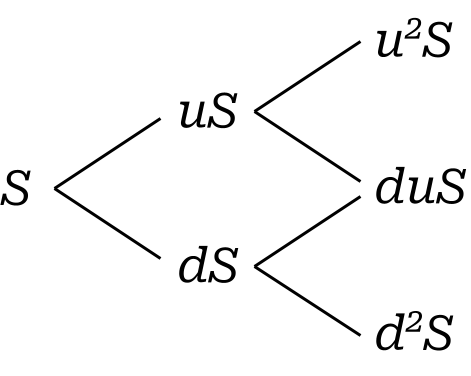
\includegraphics[height=5cm]{two-period-stock.png}
    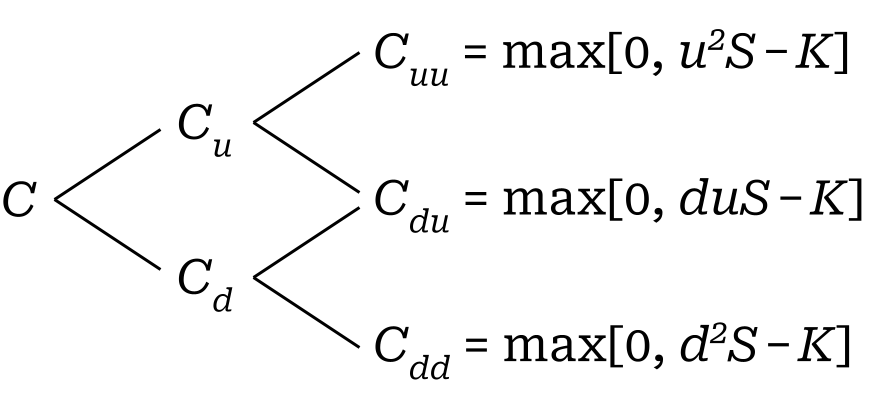
\includegraphics[height=5cm]{two-period-option.png}
    \caption{A visualization of the two-period example of the CRR model. The upper tree depicts the price paths of the underlying asset, while the lower tree depicts the paths of the (call) option value. FIX LATER WITH OWN NEW IMGS AND BETTER TEXT. IT SHOULD HAVE MORE PERIODS, AND TEXT SHOULD EXPLAIN THAT FOR PUTS YOU JUST CHANGE THE ORDER OF THE MAX. Also, make it explain the pseudocode for the algorithm as well}
    \label{fig:combined}
\end{figure}

Ganesan, Chamberlain and Buhler \cite{ganesan2009acceleration} present another approach that aims to utilize parallelism over the time-steps in addition to within them. This method focuses more on pricing a single option, and achieves parallelism over different time steps by a clever reformulation of the problem that breaks the direct dependencies between time steps. By using equation \eqref{risk-neutral-expectancy} the (European) option values at timestep $i$ are related to the prices at the next time-step $i+1$. By repeatedly substituting the same formula into itself and expanding, one obtains a general formula that relates the option values at the nodes at a previous time $i-m$ with the current time-step $i$:

\begin{equation}
    F_{i-m}(j) = e^{-m r \Delta t} \sum_{k=0}^m c_k F_i(j+k)
\label{relative-prices}
\end{equation}


where $0 \leq j \leq i-m$ are the nodes at time-step $i-m$, and the coefficients $c_k, 0 \leq k \leq m$ are the corresponding (risk-neutral) probabilities of the different possible price paths from node $j$ at time $i-m$ to the nodes $j+k$ at time $i$.Just like the one-step version computes the current value using a weighted sum (risk-neutral expected value) of the values in the future two states, this general formula extends the weighted sum to include all the nodes over several future time steps that affect its value. The coefficients in this formula follow the same recursive pattern as the option values themselves, and can be computed through backward induction. Starting from time step $t$ itself, where each coefficient represents the direct relationship of a node with itself, these coefficients are built up as we move backward in time. With each step backward, they are updated using the risk-neutral probabilities to reflect all possible paths between the two time points.
'
The key insight is that while the coefficients in this reformulation still exhibits the same sequential dependency chains between sequential time steps, they can be computed independently for different segments of the lattice. Unlike for the actual option values, there is no strict requirement for starting at the terminal nodes when calculating relative option values. Using this, the authors present the following outline of a parallel algorithm:

PSEUDO ALGORITHM

1. Divide the lattice of N time steps into p partitions, each of length N/p
2. For all partitions except the rightmost one, calculate coefficients that relate the option values at the left boundary to those at the right boundary. This is done recursively and in parallel, backtracking from the right edge to the left. Since the rightmost partition already has the option values available at its right edge (terminal nodes) we can simply compute the option prices normally here.
3. Once all partition coefficients have been calculated, use equation \eqref{relative-prices} to sequentially calculate the option value at each partition boundary, rapidly propagating towards the initial node while "skipping" many intermediate calculations.

Figure ABC depicts the algorithm.


\begin{figure}[h]
    \centering
    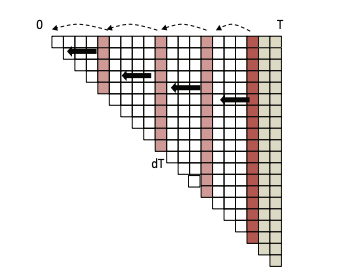
\includegraphics[height=5cm]{CRRpartitioned.png}
    \caption{A visualization of the parallelized CRR algorithm using partitioning. BLA BLA BLA lorem ipsum. MAKE YOUR OWN PICTURE OF THIS, OR CHECK IF THE FIGURES ARE OK TO USE UNDER COPYRIGHT}
    \label{fig:combined}
\end{figure}


\footnote{For what it's worth, the authors state that this can also be applied to American options by "filling in the intermediary nodes". I have been thinking about this for long now, and this still does not make sense to me. I am skeptical to claim that this is doable without having seen a better explanation on the matter. Hence, my performance analysis ignores the contribution of this step.}

Again, asymptotically, we still have $O(n^2)$ as we do computations for every node in the tree. The coefficient calculations is directly comparable to the actual option value calculations from the previous version, but we expect a factor $p$ speedup due to performing this work in parallel over all partitions. We then have to calculate the actual option values at all the nodes at the partition boundaries using \eqref{relative-prices}. The sum contains an amount of terms equal to the partition width plus one, $n/p+1$. Given enough parallel computing resources to calculate this sum for all the nodes simultaneously, this is in total an $O(n)$ operation. In practice, however, the dependency chain of the work has been reduced enough to reduce overall execution time, and the authors report a 2x speedup over a general parallel algorithm. Furthermore, they derive the optimal number of partitions $p$ for minimal execution time, and find it to be directly proportional to the square root of the amount of time steps, but inversely proportional to the square root of the latency of propagation between the partitions. Dividing the lattice into more partitions improves execution time due to parallelism up to a certain point, where the communication and boundary calculation overhead between the partitions exceed the former speedups. The paper compares this tradeoff by plotting execution time of an n=1000 size problem as a function of the number of partitions for different communication latencies (do I mention this, add it in the thesis or what?)\footnote{The original paper simplifies the analysis by only considering the communication overhead between partitions as opposed to also including the option value calculations at the boundaries. The conclusions, however, remain the same, as the choice of $p$ does not affect the computational cost of calculating the option values at the boundaries. More partitions means more boundaries to calculate in, but the smaller partition width means less summation terms. (Do I need some appendix deriving this stuff? This is my analysis based on the paper.)}.




\section{GPU Acceleration of the Black-Scholes-Merton Model} \label{sec:gpu-bsm}
\subsection{Black-Scholes-Merton Model Framework}
\subsection{European option analytical solution GPU vs CPU}
\subsection{Finite Differences numerical method for??}
\subsection{???}

\section{GPU Acceleration of Monte Carlo Methods} \label{sec:gpu-mc}
\subsection{MC in general}
\subsection{MC in options' theory}
\subsection{??????}

CONCLUSIONS TABLE WITH ALL RESULTS FROM ALL EXPERIMENTS WITH NOTES OR STANDARDIZAATION  SOMEHOW???

T\"ass\"a osassa kuvataan k\"aytetty tutkimusaineisto ja
tutkimuksen metodologiset valinnat, sek\"a
kerrotaan tutkimuksen toteutustapa ja k\"aytetyt menetelm\"at. 

\clearpage


%% Huomaa seuraavassa kappaleessa lainausmerkkien ulkopuolella piste, 
%% koska piste ei lopeta lainattua tekstinp\"atk\"a\"a.
%% Jos lainattu tekstinp\"atk\"a loppuu v\"alimerkkiin, tulee v\"alimerkki
%% lainausmerkkien sis\"alle: 
%% "Et tu, Brute?" sanoi Caesar kuollessaan.
Tutkimustuloksien merkityst\"a on aina syyt\"a arvioida ja tarkastella
kriittisesti.  Joskus tarkastelu voi olla t\"ass\"a osassa, mutta se
voidaan my\"os j\"att\"a\"a viimeiseen osaan, jolloin viimeisen osan nimeksi
tulee >>Tarkastelu>>. Tutkimustulosten merkityst\"a voi arvioida my\"os
>>Johtop\"a\"at\"okset>>-otsikon alla viimeisess\"a osassa. 

T\"ass\"a osassa on syyt\"a my\"os arvioida tutkimustulosten luotettavuutta.
Jos tutkimustulosten merkityst\"a arvioidaan >>Tarkastelu>>-osassa,
voi luotettavuuden arviointi olla my\"os siell\"a. 

\clearpage

\section{Summary}  \label{sec:summary}

\section{Conclusions}  \label{sec:conclusions}


Opinn\"aytteen tekij\"a vastaa siit\"a, ett\"a opinn\"ayte on t\"ass\"a dokumentissa
ja opinn\"aytteen tekemist\"a k\"asittelevill\"a luennoilla sek\"a
harjoituksissa annettujen ohjeiden mukainen muotoseikoiltaan,
rakenteeltaan ja ulkoasultaan.\cite{grochowski2004best}


\cleardoublepage
\phantomsection

\addcontentsline{toc}{chapter}{\bibname}
\bibliographystyle{IEEEtran}
\bibliography{bibliography.bib}


\end{document}